\chapter{Theoretical background}
\label{ch:theoretical-background}

In this chapter, we shall describe the theoretical background
taken under consideration for the developed models and analysis, including
Bayesian statistics (Section \ref{sec:bayesian_statistics}), the prevalence 
estimation problem (Section \ref{sec:prevalence_estimation_problem}), 
Respondent-driven sampling (Section \ref{sec:respodent_driven_sampling}), 
and computational methods (Section
\ref{sec:computational_methods}) used in our research. \todo{Fix order after.}

\section{Prevalence estimation problem}
\label{sec:prevalence_estimation_problem}

The study of how health-related conditions are distributed among populations
is known as {\em Epidemiology} \cite[p. 32]{rothman2008modern}, which aims to derive valid estimates for
potential causes from diseases that affect people. It is a fundamental
research area in policy formulation, implementation of prevention programs,
and development of laws. In order to accomplish these goals, the
epidemiologists use some {\em measures of disease frequency}, including {\em
incidence} and {\em prevalence}. The former is related to the proportion of
new cases of a disease given a period of time, while the latter is the proportion
of individuals exposed at time $t$ and it is the object of
study of this section. An interesting point is the following:

\begin{citacao}
  Diseases with high incidence rates may have low prevalence if they are rapidly fatal or quickly cured. Conversely, diseases with very low incidence
  rates may have substantial prevalence if they are nonfatal but incurable.
  \cite[p. 46]{rothman2008modern}
\end{citacao}

As a result, prevalence represents both incidence and the duration of disease. \textcite[p. c18]{noordzij2010measures} highlights that
prevalence reveals the burden of a disease in respect to its effects on
society, such as, monetary costs, quality of live, and morbidity. They also
comment that when measured periodically, its evolution can identify potential
causes of the infection and prevention and care methods. \todo{Should I
mention more reasons to study prevalence?} We remark that when it is impossible to test every individual at the same
time, we assume that all individuals remain exposed to the disease at time of
the last tested individual.

Consider a population of interest and a known condition, such as, for instance,
a disease or a binary behavior. A diagnostic test is done in the individuals
to measure the presence or the absence of this condition, such as serological
tests.\todo{It might be nice to add examples.} Mathematically, we denote
$\theta \in (0,1)$ the prevalence of the condition, which is the parameter of
interest. Let $I$ be a index set for the individuals. We also denote $Y^{\mathrm{true}}_i$ the indicator function of the presence of the
condition in the i$^{th}$ individual, that is, 
$$Y^{\mathrm{true}}_i = \begin{cases}
  1, &\text{if individual } i \text{ has the condition.} \\
  0, &\text{otherwise.}
\end{cases}$$

Assume for simplicity that all tests are performed at time $t$. Assume that
$Y_i$ indicates the result of the test, then 
$$Y_i = \begin{cases}
  1, &\text{if test was positive in individual } i. \\
  0, &\text{otherwise.}
\end{cases}$$

Since it is not usually feasible to test everyone in the population, it is
necessary to random select individuals from the population. On that point,
other sampling approaches may be better options, such as stratified random
sampling, systematic sampling, and two-stage cluster sampling. From that
experiment, we get a sample $\{y_1, ..., y_n\}$. Based on that outcomes the Maximum Likelihood Estimator is the following expression 
\begin{equation}
    \label{eq:naive-estimator}
    \hat{p} = \frac{1}{n}\sum_{i=1}^n y_i, 
\end{equation}
which is an estimator for the {\em apparent prevalence}, that is, the
probability of a positive outcome. 

However, this estimator assumes that the diagnostic test used is perfect,
which is often incorrect \todo{Provide some reference}. It is also not
interesting when the samples are not randomly selected (See Section
\ref{sec:respodent_driven_sampling}). From that point, it is crucial to regard
the evaluation of the diagnostic procedure by some measurement. \textcite[p.
2]{vsimundic2009measures} presents several options with different aspects,
such as the {\em likelihood ratio}, {\em sensitivity and specificity}, and
{\em the area under the ROC curve}. In this work, we consider the sensitivity
and specificity of the test. \todo{It may be good to justify this choice.}

A perfect test would discriminate every sick individual from the non-sick ones.
Given that there is not such thing, we suppose having a {\em gold standard
test}\todo{Should I cite when this not true? Cite Rutjes (2007)} that is the best available test \cite{versi1992gold} to diagnose a
particular disease. Its result is a proxy for the real $Y^{\mathrm{true}}_i$ and 

\begin{citacao}
  In the context of infectious diseases, a gold standard can be a very precise
  molecular test that detects the presence of the pathogen’s genetic material,
  polymerase chain reaction (PCR) for instance. \cite{bastos2021modelling}
\end{citacao}

From the gold standard, we can evaluate a second test, typically faster or
cheaper. The possible results upon comparing these tests are presented in
table \ref{table:two-by-two}. The definitions for each initials in the table
are the following: 

\begin{alineas}
  \item True positive (TP): when both tests agree that the individual has the
  disease. 
  \item True negative (TN): when both tests agree that the individual does not
  have the disease.
  \item False positive (FP): when the test under evaluation has a positive
  diagnose, despite the golden standard being negative. 
  \item False negative (FN): when the test under evaluation has a negative
  diagnose, despite the golden standard being positive.
\end{alineas}

\begin{table}[!ht]
  \centering
  \begin{tabular}{c|c|c|}
  \cline{2-3}
                                               & $Y = 0$ & $Y = 1$ \\ \hline
  \multicolumn{1}{|c|}{$Y^{\mathrm{true}}= 0$} & TN    & FP    \\ \hline
  \multicolumn{1}{|c|}{$Y^{\mathrm{true}}= 1$} & FN    & TP    \\ \hline
  \end{tabular}
  \caption{Two-by-two table that compares the result from the gold standard to
  the test under evaluation.}
  \label{table:two-by-two}
\end{table}

For now, we drop the index $i$ in the random variables $Y_i$ and
$Y_i^{\mathrm{true}}$. Let $p = \Pr(Y = 1)$ be the probability of a positive test.
We call $p$ the {\em apparent prevalence} since it is what the researchers 
observe. Equation \eqref{eq:naive-estimator} is an estimator for it. 
We also have that $\Pr(Y^{\mathrm{true}} = 1) = \theta$. Notice that $p$
depends on the used test, while $\theta$ does not. In prevalence estimates, we 
will only have $\theta = p$ if the test is perfect or the test is the 
gold standard itself. Define the following: 

\begin{definition}[Sensitivity]
  Probability of a positive test correctly identified. In mathematical terms,
  conditioned on $Y^{\mathrm{true}} = 1$, the {\em sensitivity} $\gamma_s$ is 
  the probability of $Y = 1$: 
  \begin{equation}
    \gamma_s = \Pr(Y = 1|Y^{\mathrm{true}} = 1). 
  \end{equation} 
\end{definition}

\begin{definition}[Specificity]
  Probability of a negative test correctly identified. In mathematical terms,
  conditioned on $Y^{\mathrm{true}} = 0$, the {\em specificity} $\gamma_e$ is 
  the probability of $Y = 0$: 
  \begin{equation}
    \gamma_e = \Pr(Y = 0|Y^{\mathrm{true}} = 0). 
  \end{equation} 
\end{definition}

\begin{theorem}[Relation between prevalence and apparent prevalence] These quantities are related by the following equation:
  \begin{equation}
    \label{eq:apparent-true-prevalence}
    p = \gamma_s\theta + (1-\gamma_e)(1-\theta).
  \end{equation}
  
\end{theorem}

\begin{proof}
  This is a direct application of the definition of conditional probability
  and the countable additivity axiom of Probability:
  \begin{equation*}
    \begin{split}
      p &= \Pr(Y = 1) = \Pr(Y = 1, Y^{\mathrm{true}} = 1) + \Pr(Y = 1, Y^{\mathrm{true}} = 0) \\
      &= \Pr(Y=1|Y^{\mathrm{true}}=1)\Pr(Y^{\mathrm{true}}=1) + \Pr(Y=1|Y^{\mathrm{true}}=0)\Pr(Y^{\mathrm{true}}=0) \\
      &= \Pr(Y=1|Y^{\mathrm{true}}=1)\Pr(Y^{\mathrm{true}}=1) \\ 
      &+ (1 - \Pr(Y=0|Y^{\mathrm{true}}=0))(1-\Pr(Y^{\mathrm{true}}=1)) \\
      &= \gamma_s\theta + (1 - \gamma_e)(1-\theta).
    \end{split}
  \end{equation*} 
\end{proof}

The intuition behind this equation is pretty simple: the proportion
of positive test counts the correct identified exposed individuals and the
incorrect identified not exposed. Equation \eqref{eq:apparent-true-prevalence}
also reveals that if $\gamma_s = \gamma_e = 1$, we have the trivial 
case $p = \theta$. Moreover, if $\gamma_s = \gamma_e = 0.5$, we have that
$p = 0.5$ and there is no information about $\theta$. 

A frequentist approach assumes that $\theta$ is fixed and unknown. Its
inference is based on the point 
estimate for the apparent prevalence $\hat{p}$ given in Equation
\eqref{eq:naive-estimator}, along with a Confidence Interval, such as the Wald
Confidence Interval built with a normal approximation. In order to provide a 
point estimate for $\hat{\theta}$, \textcite[p. 73]{rogan1978estimating} propose
$$\hat{\theta}^{RG} = \frac{\hat{p} - (1-\gamma_e)}{\gamma_s + \gamma_e -
1}.$$ 
Suppose a disease with prevalence $\theta = 0.01$. In this case, we would have
that $p \approx 1 - \gamma_e$ by equation \eqref{eq:apparent-true-prevalence}.
Given the randomness, it is possible to have $\hat{p} < 1 - \gamma_e$, which
would define a useless estimative for $\theta$. Besides that, Confidence Intervals for that 
expression does not include uncertainty about $\gamma_e$ and $\gamma_s$. On
the other side, a Bayesian approach let $\theta$ be a random variable,
allowing the researcher to incorporate their uncertainty on the prior
distribution, which is explained in Section
\ref{sec:bayesian_statistics}. It also allows to include uncertainty in
sensitivity and specificity of the test. According to \textcite[p.
1]{branscum2005estimation}:
\begin{citacao}
  Diagnostic-test evaluation is particularly suited to the
  Bayesian framework because prior scientific information about the
  sensitivities and specificities of the tests and prior information about the prevalences of the sampled
  populations can be incorporated.
\end{citacao}

Therefore, this work focus on the Bayesian paradigm.

\section{Respondent-driven sampling}
\label{sec:respodent_driven_sampling}

Respondent-driven sampling (RDS) is a procedure developed by Heckathorn
\cite[]{heckathorn1997} to survey {\em hidden} or {\em hard-to-reach
populations}, whose main characteristic is the absence of a sampling frame,
i.e.,it is not possible to enumerate its individuals since size and boundaries
are unknown. The second characteristic of these populations is the
confidentiality concerns, given that membership is stigmatized or illegal.
With that aspect, traditional sampling methods which produce probability
samples are infeasible. To overcome this, Snowball Sampling \cite[]{goodman1961}
is the most common method, and it relies on the respondents to nominate more 
subjects within the population as a snowball. Examples of studied groups
include people who inject drugs (PWID), men who have sex with men (MSM), and
female sex workers (FSW) \cite[p. 66]{gile2018methods}. 

Heckathorn's proposal \citeyear{heckathorn1997} was to specialize this method without the need of
nominating peers. In this approach, the researchers select some individuals,
called {\em seeds} from the target population, and give them a fixed amount of
{\em recruitment coupons} to recruit their peers. Each recipient of the coupons
reclaims it in the study site, is interviewed, and receives more coupons to
continue the recruitment. This process occurs until it reaches some stopping
criteria, such as the sample size achieving some desired number. The sampling
is without replacement, so the participants cannot be recruited more than
once. Moreover, the respondents inform how many subjects from the population
they know. Other less usual methods include Key Important Sampling \cite{deaux-callaghan1985}, 
and Targeted Sampling \cite{watters-biernacki1989}, both are convenience
sampling methods. 

According to \textcite[p. 66]{gile2018methods}, there are two main advantages
of RDS over other snowball samplings. First, the fixed number of recruitment
coupons enforces the network gets deeper and distant from the seeds, which
reduces the dependence of the final sample from the initial chosen by
researchers. Second, since the recruited subjects do not have to name their
peers, confidentiality is maintained until the recruitment is completed.
Other problems cited by \textcite[p. 175]{heckathorn1997} include biases
towards individuals who are more cooperative, biases by masking when the
participants do not name friends for the next wave to protect them, and
individuals with more links may be oversampled. RDS offers a solution with a
{\em dual incentive system}, explained in Subsection
\ref{sec:sampling-procedure}. 

Since the creation of the method by Heckathorn, several papers have been
published as \autoref{fig:chart-research-rds} presents. The figure was
produced searching publications with the term ``Respondent driven sampling''.
These works generally aim to give basis to public health policies. Good
examples in Brazil are \cite{damacena2019application}, which applies RDS
method to carry out a biological and behavioral surveillance in FSW
populations from twelve cities in Brazil; \cite{mota2012respondent},
which proposes to apply RDS method in MSM populations from ten cites in Brazil,
and \cite{bastos2018hiv}, which studies several sexual transmitted infection
among transgender women from twelve brazilian cities. 

\begin{figure}
  \centering  
  \caption{\label{fig:chart-research-rds}Publications by year with the term
  ``Respondent driven sampling'' from 1997 to 2021.}
  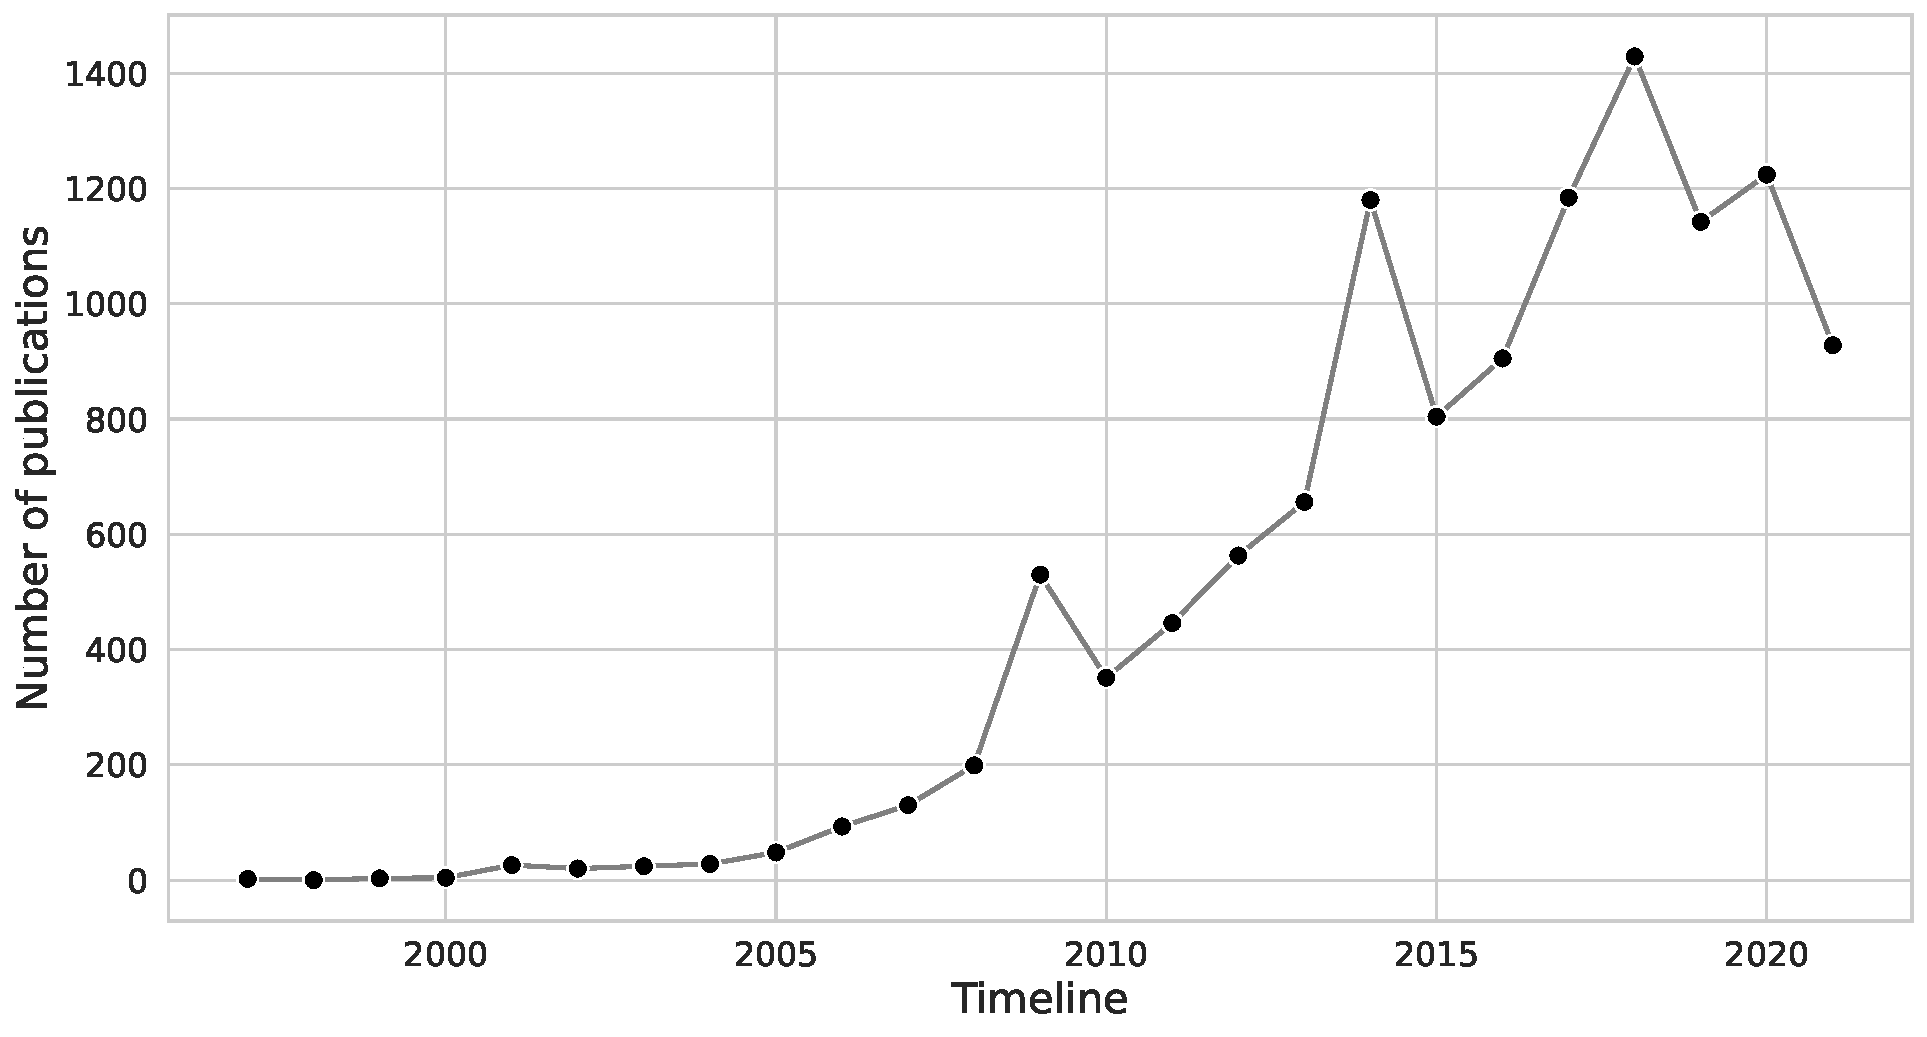
\includegraphics[width=14cm]{chart_research_growing_rds.pdf}
  \fonte{htpps://app.dimensions.ai. Exported on October 31, 2021.}
\end{figure}

\subsection{Details about the sampling procedure}
\label{sec:sampling-procedure}

The RDS method was expanded by \textcite{heckathorn2002}. It detailed two aspects: 
introducing a way to correct {\em homophily} biases that is the tendency for
individuals to connect to others similar to them, and {\em personal network size} or
{\em degree} that is the number of connections of an individual within the
target population. It also presented a bootstrapping procedure to quantify
uncertainty about inferences. The procedure was slightly modified by
\textcite{salganik2004sampling} with a proof that under some regularity
conditions, RDS estimators were asymptotically unbiased. Examples of questions
about personal degree are the following: 

How seeds are selected and explain the number of coupons. Why is it fixed? Why
is it three? "This number is chosen to strike a balance between the inferential
desire to limit the branching of the sample and the practical necessity of guarding against the early
termination of the sample trees". 

The subjects receive a reward for being interviewed and for each recruitment
of their peers which establishes a dual incentive system. The {\em primary incentive} is the
{\em individual-sanction-based control}, so there is a reward for
participating. The second one is the {\em group-mediated social control} that
influences the participants to induce others to comply to get the reward for the recruitment. When social approval is important, recruitment can be even
more efficient and cheaper, since material incentive can be converted into
symbolic by the individuals. In summary, accepting to be recruited will have a
material incentive for both and a symbolic incentive for the recruited, since
theirs peers also participated.

\subsection{Assumptions and statistical properties}

Clustering and homophily: extent to which people have connections with
‘like’ people (27); Hx = 2pi(1 - pi)R - 1

\subsection{Models for the RDS Process}

Although regression analysis of RDS data is frequently undertaken, the best method for accommodating
  correlation between participants (clustering) and the non-random sampling of
  recruits remains unknown."

\subsubsection{Markov process}

Describe as a Markov process \cite{heckathorn1997}

\subsubsection{Random walk}

\cite{heckathorn2002} Actually if was 2004. 

\subsubsection{Graphical model}

Let $G = (V,E)$ be an undirected graph representing the hidden population. The {\em recruitment graph} $G_R =
(V_R, E_R)$ represents the recruited individuals and the recruitment edges,
that is, $(i,j) \in E_R$ if, and only if, $i$ recruited $j$.
Given that each individual can be sampled only once, it is not possible to
observe the {\em recruitment-induced subgraph}, that is the induced subgraph
generated by $V_R$. Moreover, the {\em coupon matrix} $C$ defined by $C_{ij} =
1$ if the i$^{th}$ subject has at least one coupon before the j$^{th}$
recruitment event, is also observed with the recruitment times. Assuming an
exponential and independent distribution of the times, the likelihood can be
written explicitly, and the distribution interpreted as an exponential random graph
model \cite[]{crawford2016}.  

These models allowed several applications in social sciences, epidemiology,
and statistics, including hidden populations size estimation
\cite[]{crawford2018hidden}, regression \cite[]{bastos2012binary}, communicable
disease prevalence estimation \cite[]{albuquerque2009avaliaccao}, among
others.

\subsubsection{New model}

Present the non-read-yet model. 

\subsection{Prevalence estimators}

Review of RDS prevalence estimators: naive estimator; RDS-I estimator;
RDS-II; Gile SS; HCG estimator;

weighting of those with more connections; 

GLM procedures cited!

\subsection{Regression methods}

"A search of PubMed for the terms ‘respondent driven sampling’ and
‘regression’"

Regression techniques that already exist: weighted regression (33-37);

\section{Generalized linear models}
\label{sec:glm}

Generalized linear models are an extension of classical linear models. 
Let $y \in \R^{n}$ be a realization of a random variable 
$Y : \Omega \to \mathbb{R}^n$ associated with a phenomena such that each 
component $Y_i$ is independent of the others. The systematic process in 
modelling is the specification of the vector $\mu = \ev[Y]$ through a small 
number of parameters $\beta_1, \dots, \beta_p$. The classical linear model 
assumes that $Y_i \overset{iid}{\sim} \N(\mu_i, \sigma^2)$ and $\mu = X\beta$,
where $X \in \R^{n \times p}$ is the data, where $X_{ij}$ is the measure 
of the $j$-th covariate in the $i$-th individual. 

The main generalization of this aspect is the introduction of the 
\textit{link function}. This is a monotonic differentiable function $g$ 
such that $\eta_i = g(\mu_i)$ and $\eta = X\beta$. Therefore the link 
function relates the linear predictor $\eta$ to the expected value $\mu$. 
The distribution of $Y$ 
may also come from another exponential family distribution \todo{Maybe 
explain or cite what is this?}

Classical link functions when $Y_i$ has Binomial distribution with 
parameter $0 < \mu < 1$ are 

\begin{enumerate}
  \item \textit{logit}: $\eta = \log(\mu / (1 - \mu))$ that represents 
  the log odds of $Y_i = 1$. 
  \item \textit{probit}: $\eta = \Phi^{-1}(\mu)$ where the $\Phi(\cdot)$ 
  is the Normal cumulative distribution function; 
  \item \textit{complementary log-log}: $\eta = \log(-\log(1 - \mu))$.
\end{enumerate}


\section{Bayesian statistics}
\label{sec:bayesian_statistics}

We can represent our beliefs and information about unknown quantities 
through probabilities. There are two more common interpretations: 
frequentist and Bayesian. While the frequentists define
probability as the limit of a frequency in a large number of trials, the
Bayesians represent an individual's degree of belief in a statement that is
updated given new information. This philosophy allows assigning probabilities
to any event, even if a random process is not defined \cite{statisticat2016laplacesdemon}. 

In 1761, Reverend Thomas Bayes wrote for the first time the Bayes' formula
relating the probability of a parameter after observing the data with the
evidence (written through a likelihood function) and previous information
about the parameter. Pierre Simon Laplace rediscovered this formula in 1773
\cite{Robert2007}, and this theory became more common in the 19th century.
After some criticisms, a modern treatment considering Kolmogorov's
axiomatization of the theory of probabilities started after Jeffreys in 1939.
The recent development of new computational tools brought these ideas again.

Therefore, Bayesian inference is the process of inductive learning using
Bayes' rule, where inductive means that characteristics of a population are 
learned from a subset of it. We generally
express numerical characteristics of the population as a parameter $\theta$ which is
indirectly observed through numerical descriptions $y$ of the population. Both are
uncertain until the observation of a sample, when its information can decrease
our uncertainty about the population characteristics \cite[p. 1-2]{hoff2009first}.

The set of all possible outcomes $y$ forms the {\em sample space}
$\mathcal{Y}$, while the set of all possible parameters forms the {\em
parameter space} $\Theta$. Bayesian inference is composed by the following: 

\begin{enumerate}[label=(\alph*)]
    \item {\em Prior distribution:} A probability distribution defined over 
    $\Theta$ that quantifies our beliefs about $\theta$ before observing the data;
    \item {\em Sampling model: } A probability distribution of the data generation process
    that express our belief that $y \in \mathcal{Y}$ is the outcome when
    $\theta \in \Theta$ is true. When it is seen as function of the parameter,
    it is called {\em likelihood function};
    \item {\em Loss function:} Only in a decision theory framework, it
    measures the error of a estimative $\delta \in \Theta$ in comparison to
    $\theta$. 
    \item {\em Posterior distribution:} Once we get the data $y$, it
    represents our updated beliefs out the parameter conditioned All
    inferences are based on this probability distribution.
\end{enumerate} 

Bayes' theorem establishes that when the sampling model is absolutely
continuous with respect to some measure $\nu$ with conditional density
$f_{Y\mid \theta}(y\mid\theta)$ and the prior distribution is a
well defined probability measure $\mu_{\theta}$, the posterior distribution
$\mu_{\theta|Y}(\cdot\mid y)$ is
absolutely continuous with respect to $\mu_{\theta}$ almost surely and its
Radon-Nikodym derivative is \cite[p. 16]{schervish2012theory}
\begin{equation}
  \label{eq:bayes-update-measure}
  \frac{d\mu_{\theta\mid Y}}{d\mu_{\theta}}(\theta|y) = \frac{f_{Y\mid \theta}(y\mid \theta)}{\int_{\Theta} f_{Y\mid\theta}(y|t)d\mu_{\theta}(t)}.  
\end{equation}

When the prior distribution is absolutely continuous with respect to the
Lebesgue measure, equation \eqref{eq:bayes-update-measure} resumes to 
\begin{equation}
  p(y|\theta) = \frac{f(y\mid \theta)\pi(\theta)}{\int_{\Theta} f(y\mid t)\pi(t) \, dt}.  
\end{equation}

\section{Computational methods}
\label{sec:computational_methods}

\subsection{Hamiltonian Monte Carlo}
\label{sec:hamiltonian-monte-carlo}

We follow \cite{betancourt2017conceptual}. This method was developed in the late 1980s as Hybrid Monte Carlo to tackle calculations in Lattice Quantum Chromodynamics. Instead of moving in the parameter space randomly with uninformed jumps, the direction from the vector field given by the gradients are used to trace out a trajectory through the *typical set*, the region which has significant contribution to the expectations. However, if only the gradient was used, the trajectory would pull towards the mode of the distribution, so more geometric constraints are needed. In order to a satellite rotate around the Earth, we have to endow ir with enough momentum to counteract the gravitational field, turning the system into a conservative one. 

First, we introduce auxiliary momentum parameters $p_n$ (lift) of the same dimension from the parameter space $\Omega \subseteq \mathbb{R}^D$. Then $q_n$ turns to $(q_n, p_n)$, with the use the joint probability distribution $\pi(q,p) = \pi(p\mid q)\pi(q)$. Particularly, we use 

$$
\pi(q,p) = e^{-H(q,p)}, 
$$

such that $H$ is the *Hamiltonian*. Note that $H(q,p) = -\log \pi(p\mid q) - \log \pi(q) =: K(p,q) + V(q)$. We call $K$ the kinetic energy, and $V$ the potential energy. The vector field is generated by Hamilton's equations, 

$$
\frac{dq}{dt} = \frac{\partial H}{\partial p} = \frac{\partial K}{\partial p}
$$
$$
\frac{dp}{dt} = -\frac{\partial H}{\partial q} = -\frac{\partial K}{\partial q} - \frac{d V}{d q}.
$$

Therefore, we are able to define the Hamiltonian flows $\phi_t : (p,q) \to
(p,q), \forall t \in \mathbb{R}$.

\subsubsection{Diagnostics}

The importance of diagnosing. The potential problems that it can show. 

\begin{itemize}
  \item Divergent transitions; 
  \item Transitions that hit the maximum tree depth; 
  \item Low E-BFMI values; 
  \item Low effective samples sizes; 
  \item $\hat{R} \not \in (0.95, 1.05)$.   
\end{itemize}